% Created by tikzDevice version 0.12.6 on 2024-02-19 14:19:22
% !TEX encoding = UTF-8 Unicode
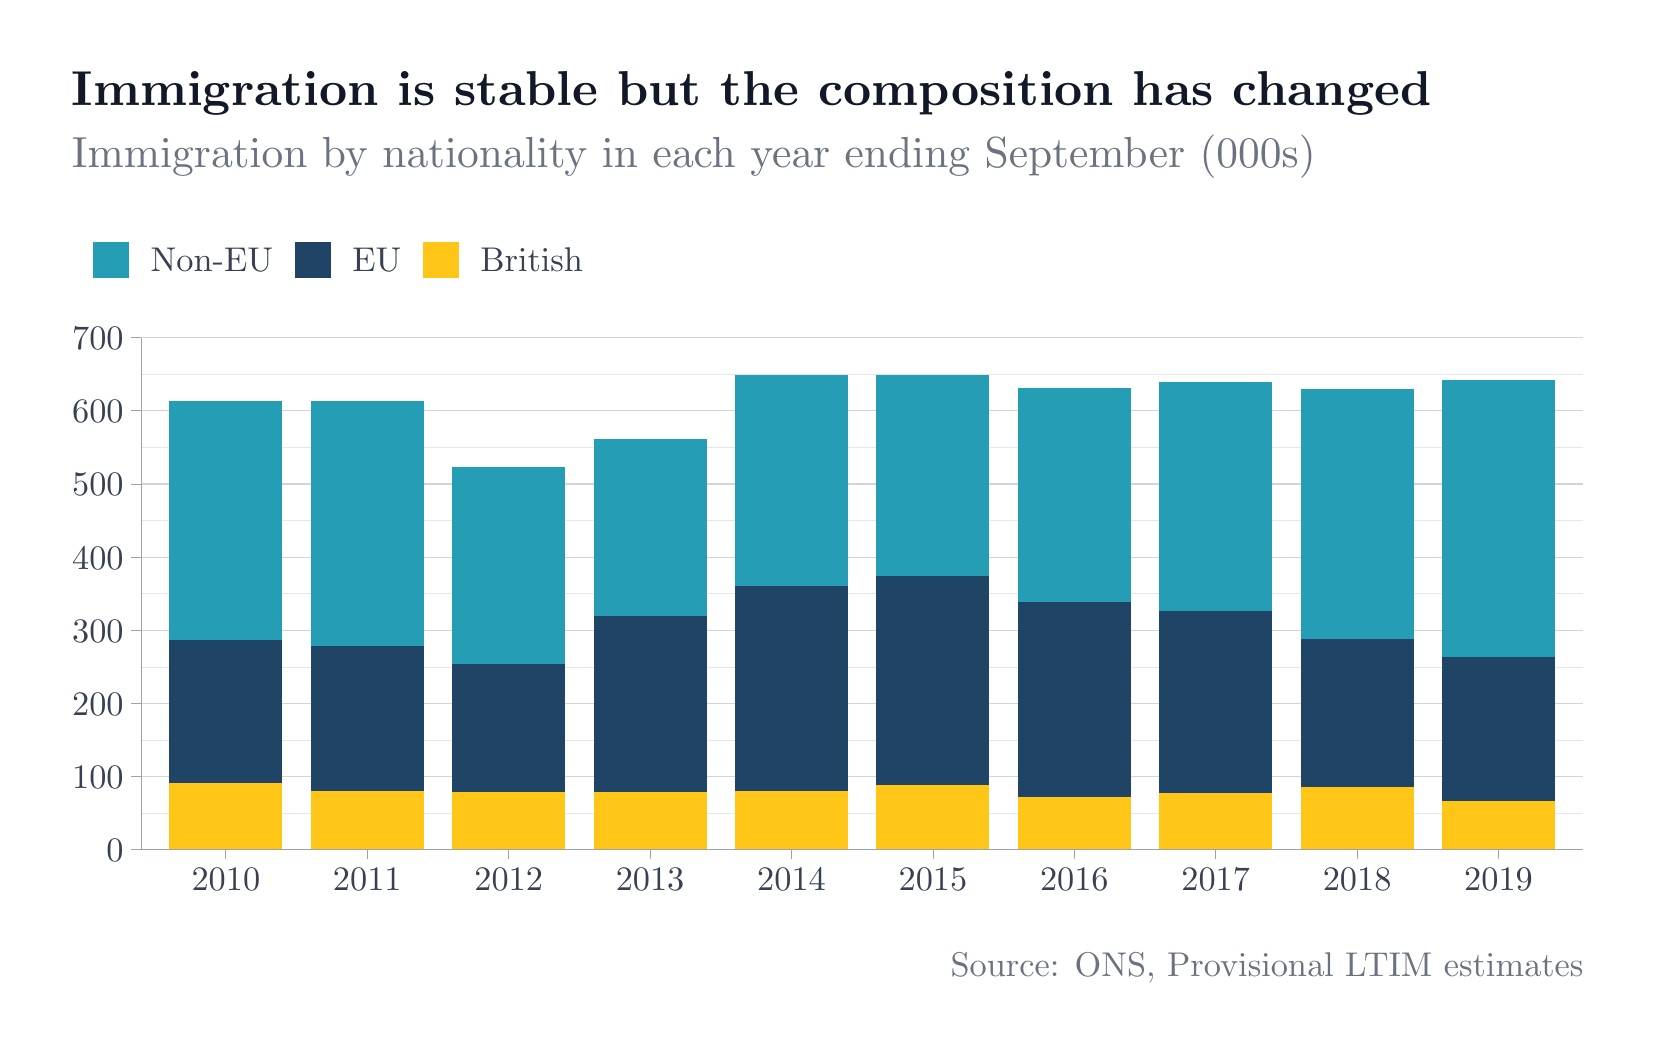
\begin{tikzpicture}[x=1pt,y=1pt]
\definecolor{fillColor}{RGB}{255,255,255}
\path[use as bounding box,fill=fillColor] (0,0) rectangle (578.16,361.35);
\begin{scope}
\path[clip] (  0.00,  0.00) rectangle (578.16,361.35);
\definecolor{drawColor}{RGB}{255,255,255}

\path[draw=drawColor,line width= 0.7pt,line join=round,line cap=round,fill=fillColor] (  0.00,  0.00) rectangle (578.16,361.35);
\end{scope}
\begin{scope}
\path[clip] ( 40.96, 64.27) rectangle (562.16,249.31);
\definecolor{drawColor}{RGB}{255,255,255}
\definecolor{fillColor}{RGB}{255,255,255}

\path[draw=drawColor,line width= 0.7pt,line join=round,line cap=round,fill=fillColor] ( 40.96, 64.27) rectangle (562.16,249.31);
\definecolor{drawColor}{RGB}{229,231,235}

\path[draw=drawColor,line width= 0.2pt,line join=round] ( 40.96, 77.49) --
	(562.16, 77.49);

\path[draw=drawColor,line width= 0.2pt,line join=round] ( 40.96,103.92) --
	(562.16,103.92);

\path[draw=drawColor,line width= 0.2pt,line join=round] ( 40.96,130.36) --
	(562.16,130.36);

\path[draw=drawColor,line width= 0.2pt,line join=round] ( 40.96,156.79) --
	(562.16,156.79);

\path[draw=drawColor,line width= 0.2pt,line join=round] ( 40.96,183.23) --
	(562.16,183.23);

\path[draw=drawColor,line width= 0.2pt,line join=round] ( 40.96,209.66) --
	(562.16,209.66);

\path[draw=drawColor,line width= 0.2pt,line join=round] ( 40.96,236.10) --
	(562.16,236.10);
\definecolor{drawColor}{RGB}{209,213,219}

\path[draw=drawColor,line width= 0.4pt,line join=round] ( 40.96, 64.27) --
	(562.16, 64.27);

\path[draw=drawColor,line width= 0.4pt,line join=round] ( 40.96, 90.71) --
	(562.16, 90.71);

\path[draw=drawColor,line width= 0.4pt,line join=round] ( 40.96,117.14) --
	(562.16,117.14);

\path[draw=drawColor,line width= 0.4pt,line join=round] ( 40.96,143.58) --
	(562.16,143.58);

\path[draw=drawColor,line width= 0.4pt,line join=round] ( 40.96,170.01) --
	(562.16,170.01);

\path[draw=drawColor,line width= 0.4pt,line join=round] ( 40.96,196.44) --
	(562.16,196.44);

\path[draw=drawColor,line width= 0.4pt,line join=round] ( 40.96,222.88) --
	(562.16,222.88);

\path[draw=drawColor,line width= 0.4pt,line join=round] ( 40.96,249.31) --
	(562.16,249.31);
\definecolor{fillColor}{RGB}{255,197,23}

\path[fill=fillColor] ( 51.18, 64.27) rectangle ( 92.05, 88.59);

\path[fill=fillColor] (102.27, 64.27) rectangle (143.15, 85.68);

\path[fill=fillColor] (153.37, 64.27) rectangle (194.25, 85.16);

\path[fill=fillColor] (204.47, 64.27) rectangle (245.35, 85.16);

\path[fill=fillColor] (255.57, 64.27) rectangle (296.45, 85.68);

\path[fill=fillColor] (306.67, 64.27) rectangle (347.55, 87.53);

\path[fill=fillColor] (357.77, 64.27) rectangle (398.64, 83.30);

\path[fill=fillColor] (408.86, 64.27) rectangle (449.74, 84.89);

\path[fill=fillColor] (459.96, 64.27) rectangle (500.84, 87.01);

\path[fill=fillColor] (511.06, 64.27) rectangle (551.94, 81.98);
\definecolor{fillColor}{RGB}{32,68,102}

\path[fill=fillColor] ( 51.18, 88.59) rectangle ( 92.05,140.14);

\path[fill=fillColor] (102.27, 85.68) rectangle (143.15,138.02);

\path[fill=fillColor] (153.37, 85.16) rectangle (194.25,131.42);

\path[fill=fillColor] (204.47, 85.16) rectangle (245.35,148.86);

\path[fill=fillColor] (255.57, 85.68) rectangle (296.45,159.44);

\path[fill=fillColor] (306.67, 87.53) rectangle (347.55,163.14);

\path[fill=fillColor] (357.77, 83.30) rectangle (398.64,153.88);

\path[fill=fillColor] (408.86, 84.89) rectangle (449.74,150.45);

\path[fill=fillColor] (459.96, 87.01) rectangle (500.84,140.40);

\path[fill=fillColor] (511.06, 81.98) rectangle (551.94,133.79);
\definecolor{fillColor}{RGB}{36,157,181}

\path[fill=fillColor] ( 51.18,140.14) rectangle ( 92.05,226.32);

\path[fill=fillColor] (102.27,138.02) rectangle (143.15,226.32);

\path[fill=fillColor] (153.37,131.42) rectangle (194.25,202.52);

\path[fill=fillColor] (204.47,148.86) rectangle (245.35,212.83);

\path[fill=fillColor] (255.57,159.44) rectangle (296.45,235.83);

\path[fill=fillColor] (306.67,163.14) rectangle (347.55,235.83);

\path[fill=fillColor] (357.77,153.88) rectangle (398.64,231.07);

\path[fill=fillColor] (408.86,150.45) rectangle (449.74,233.45);

\path[fill=fillColor] (459.96,140.40) rectangle (500.84,230.81);

\path[fill=fillColor] (511.06,133.79) rectangle (551.94,233.98);

\path[] ( 40.96, 64.27) rectangle (562.16,249.31);
\end{scope}
\begin{scope}
\path[clip] (  0.00,  0.00) rectangle (578.16,361.35);
\definecolor{drawColor}{RGB}{156,163,175}

\path[draw=drawColor,line width= 0.3pt,line join=round] ( 40.96, 64.27) --
	( 40.96,249.31);
\end{scope}
\begin{scope}
\path[clip] (  0.00,  0.00) rectangle (578.16,361.35);
\definecolor{drawColor}{RGB}{55,65,81}

\node[text=drawColor,anchor=base east,inner sep=0pt, outer sep=0pt, scale=  1.24] at ( 34.66, 59.99) {0};

\node[text=drawColor,anchor=base east,inner sep=0pt, outer sep=0pt, scale=  1.24] at ( 34.66, 86.42) {100};

\node[text=drawColor,anchor=base east,inner sep=0pt, outer sep=0pt, scale=  1.24] at ( 34.66,112.86) {200};

\node[text=drawColor,anchor=base east,inner sep=0pt, outer sep=0pt, scale=  1.24] at ( 34.66,139.29) {300};

\node[text=drawColor,anchor=base east,inner sep=0pt, outer sep=0pt, scale=  1.24] at ( 34.66,165.73) {400};

\node[text=drawColor,anchor=base east,inner sep=0pt, outer sep=0pt, scale=  1.24] at ( 34.66,192.16) {500};

\node[text=drawColor,anchor=base east,inner sep=0pt, outer sep=0pt, scale=  1.24] at ( 34.66,218.60) {600};

\node[text=drawColor,anchor=base east,inner sep=0pt, outer sep=0pt, scale=  1.24] at ( 34.66,245.03) {700};
\end{scope}
\begin{scope}
\path[clip] (  0.00,  0.00) rectangle (578.16,361.35);
\definecolor{drawColor}{RGB}{156,163,175}

\path[draw=drawColor,line width= 0.3pt,line join=round] ( 37.46, 64.27) --
	( 40.96, 64.27);

\path[draw=drawColor,line width= 0.3pt,line join=round] ( 37.46, 90.71) --
	( 40.96, 90.71);

\path[draw=drawColor,line width= 0.3pt,line join=round] ( 37.46,117.14) --
	( 40.96,117.14);

\path[draw=drawColor,line width= 0.3pt,line join=round] ( 37.46,143.58) --
	( 40.96,143.58);

\path[draw=drawColor,line width= 0.3pt,line join=round] ( 37.46,170.01) --
	( 40.96,170.01);

\path[draw=drawColor,line width= 0.3pt,line join=round] ( 37.46,196.44) --
	( 40.96,196.44);

\path[draw=drawColor,line width= 0.3pt,line join=round] ( 37.46,222.88) --
	( 40.96,222.88);

\path[draw=drawColor,line width= 0.3pt,line join=round] ( 37.46,249.31) --
	( 40.96,249.31);
\end{scope}
\begin{scope}
\path[clip] (  0.00,  0.00) rectangle (578.16,361.35);
\definecolor{drawColor}{RGB}{156,163,175}

\path[draw=drawColor,line width= 0.3pt,line join=round] ( 40.96, 64.27) --
	(562.16, 64.27);
\end{scope}
\begin{scope}
\path[clip] (  0.00,  0.00) rectangle (578.16,361.35);
\definecolor{drawColor}{RGB}{156,163,175}

\path[draw=drawColor,line width= 0.3pt,line join=round] ( 71.61, 60.77) --
	( 71.61, 64.27);

\path[draw=drawColor,line width= 0.3pt,line join=round] (122.71, 60.77) --
	(122.71, 64.27);

\path[draw=drawColor,line width= 0.3pt,line join=round] (173.81, 60.77) --
	(173.81, 64.27);

\path[draw=drawColor,line width= 0.3pt,line join=round] (224.91, 60.77) --
	(224.91, 64.27);

\path[draw=drawColor,line width= 0.3pt,line join=round] (276.01, 60.77) --
	(276.01, 64.27);

\path[draw=drawColor,line width= 0.3pt,line join=round] (327.11, 60.77) --
	(327.11, 64.27);

\path[draw=drawColor,line width= 0.3pt,line join=round] (378.21, 60.77) --
	(378.21, 64.27);

\path[draw=drawColor,line width= 0.3pt,line join=round] (429.30, 60.77) --
	(429.30, 64.27);

\path[draw=drawColor,line width= 0.3pt,line join=round] (480.40, 60.77) --
	(480.40, 64.27);

\path[draw=drawColor,line width= 0.3pt,line join=round] (531.50, 60.77) --
	(531.50, 64.27);
\end{scope}
\begin{scope}
\path[clip] (  0.00,  0.00) rectangle (578.16,361.35);
\definecolor{drawColor}{RGB}{55,65,81}

\node[text=drawColor,anchor=base,inner sep=0pt, outer sep=0pt, scale=  1.24] at ( 71.61, 49.40) {2010};

\node[text=drawColor,anchor=base,inner sep=0pt, outer sep=0pt, scale=  1.24] at (122.71, 49.40) {2011};

\node[text=drawColor,anchor=base,inner sep=0pt, outer sep=0pt, scale=  1.24] at (173.81, 49.40) {2012};

\node[text=drawColor,anchor=base,inner sep=0pt, outer sep=0pt, scale=  1.24] at (224.91, 49.40) {2013};

\node[text=drawColor,anchor=base,inner sep=0pt, outer sep=0pt, scale=  1.24] at (276.01, 49.40) {2014};

\node[text=drawColor,anchor=base,inner sep=0pt, outer sep=0pt, scale=  1.24] at (327.11, 49.40) {2015};

\node[text=drawColor,anchor=base,inner sep=0pt, outer sep=0pt, scale=  1.24] at (378.21, 49.40) {2016};

\node[text=drawColor,anchor=base,inner sep=0pt, outer sep=0pt, scale=  1.24] at (429.30, 49.40) {2017};

\node[text=drawColor,anchor=base,inner sep=0pt, outer sep=0pt, scale=  1.24] at (480.40, 49.40) {2018};

\node[text=drawColor,anchor=base,inner sep=0pt, outer sep=0pt, scale=  1.24] at (531.50, 49.40) {2019};
\end{scope}
\begin{scope}
\path[clip] (  0.00,  0.00) rectangle (578.16,361.35);
\definecolor{fillColor}{RGB}{255,255,255}

\path[fill=fillColor] ( 16.00,263.31) rectangle (207.79,291.77);
\end{scope}
\begin{scope}
\path[clip] (  0.00,  0.00) rectangle (578.16,361.35);
\definecolor{drawColor}{RGB}{255,255,255}
\definecolor{fillColor}{RGB}{255,255,255}

\path[draw=drawColor,line width= 0.7pt,line join=round,line cap=round,fill=fillColor] ( 23.00,270.31) rectangle ( 37.45,284.77);
\end{scope}
\begin{scope}
\path[clip] (  0.00,  0.00) rectangle (578.16,361.35);
\definecolor{fillColor}{RGB}{36,157,181}

\path[fill=fillColor] ( 23.71,271.02) rectangle ( 36.74,284.06);
\end{scope}
\begin{scope}
\path[clip] (  0.00,  0.00) rectangle (578.16,361.35);
\definecolor{drawColor}{RGB}{255,255,255}
\definecolor{fillColor}{RGB}{255,255,255}

\path[draw=drawColor,line width= 0.7pt,line join=round,line cap=round,fill=fillColor] ( 95.85,270.31) rectangle (110.30,284.77);
\end{scope}
\begin{scope}
\path[clip] (  0.00,  0.00) rectangle (578.16,361.35);
\definecolor{fillColor}{RGB}{32,68,102}

\path[fill=fillColor] ( 96.56,271.02) rectangle (109.59,284.06);
\end{scope}
\begin{scope}
\path[clip] (  0.00,  0.00) rectangle (578.16,361.35);
\definecolor{drawColor}{RGB}{255,255,255}
\definecolor{fillColor}{RGB}{255,255,255}

\path[draw=drawColor,line width= 0.7pt,line join=round,line cap=round,fill=fillColor] (142.09,270.31) rectangle (156.55,284.77);
\end{scope}
\begin{scope}
\path[clip] (  0.00,  0.00) rectangle (578.16,361.35);
\definecolor{fillColor}{RGB}{255,197,23}

\path[fill=fillColor] (142.80,271.02) rectangle (155.84,284.06);
\end{scope}
\begin{scope}
\path[clip] (  0.00,  0.00) rectangle (578.16,361.35);
\definecolor{drawColor}{RGB}{55,65,81}

\node[text=drawColor,anchor=base west,inner sep=0pt, outer sep=0pt, scale=  1.24] at ( 44.45,273.26) {Non-EU};
\end{scope}
\begin{scope}
\path[clip] (  0.00,  0.00) rectangle (578.16,361.35);
\definecolor{drawColor}{RGB}{55,65,81}

\node[text=drawColor,anchor=base west,inner sep=0pt, outer sep=0pt, scale=  1.24] at (117.30,273.26) {EU};
\end{scope}
\begin{scope}
\path[clip] (  0.00,  0.00) rectangle (578.16,361.35);
\definecolor{drawColor}{RGB}{55,65,81}

\node[text=drawColor,anchor=base west,inner sep=0pt, outer sep=0pt, scale=  1.24] at (163.55,273.26) {British};
\end{scope}
\begin{scope}
\path[clip] (  0.00,  0.00) rectangle (578.16,361.35);
\definecolor{drawColor}{RGB}{107,114,128}

\node[text=drawColor,anchor=base west,inner sep=0pt, outer sep=0pt, scale=  1.57] at ( 16.00,310.83) {Immigration by nationality in each year ending September (000s)};
\end{scope}
\begin{scope}
\path[clip] (  0.00,  0.00) rectangle (578.16,361.35);
\definecolor{drawColor}{RGB}{17,24,39}

\node[text=drawColor,anchor=base west,inner sep=0pt, outer sep=0pt, scale=  1.77] at ( 16.00,333.12) {\bfseries Immigration is stable but the composition has changed};
\end{scope}
\begin{scope}
\path[clip] (  0.00,  0.00) rectangle (578.16,361.35);
\definecolor{drawColor}{RGB}{107,114,128}

\node[text=drawColor,anchor=base east,inner sep=0pt, outer sep=0pt, scale=  1.24] at (562.16, 18.42) {Source: ONS, Provisional LTIM estimates};
\end{scope}
\end{tikzpicture}
